For the results we are going look at the different approaches for a quantum beauty contest, considering variation of parameters, and investigate special behavior while comparing this to the classical results from lab studies. When talking about the expected value of $\ket{\psi}$ or $\ket{S}$ in the following we will only refer to the values where no contraction factor $p$ has been applied yet, if not stated otherwise.\\

\subsection{The Semi Classical Approach}
\label{sub: The semi classical approach}

First we look at the approach where the winning state $\ket{w}$ is determined from the expected value of $\ket{\psi}$ and the fitness of $\ket{\text{S}_i}$ is determined by its distance of its expected value to $\ket{w}$. This approach is almost identical to the classical game. The main difference are the real values of the expectation from each player. For any simulation these are still rational numbers due to the machines precision of values. An analogue for the classical game could therefore be the formation of alliances of players which then give their average as a guess. In the edge case of an infinite amount of players in an alliance we could still reproduce real numbers as a guess. As this approach is almost isomorphic to the classical game, we expect a similar approach to $\ket{0}$ for $\ket{w}$. While we do observe this as seen in figure \ref{fig:avg_avg_exp_val}, we do not quite reach a state of 0 after many iterations, which is due to our evolution algorithm allowing for relatively strong mutations, even for high states. An analogue to this in the classical game might be a disruptive player who purposefully chooses numbers that can not win ($n\cdot p$ or above) after several rounds, which can also be seen in \ref{fig:1}.

\begin{figure}[h]
    \centering
    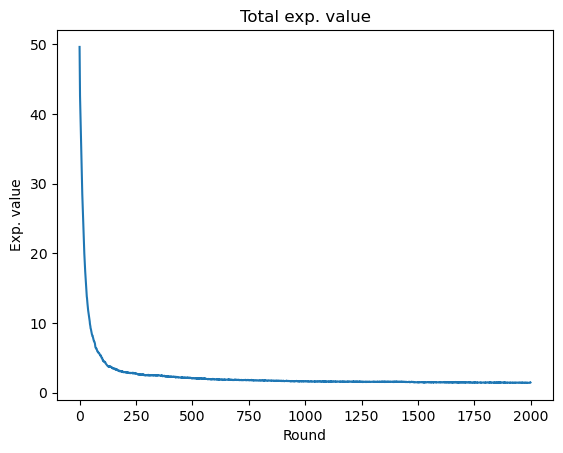
\includegraphics[width=0.45\textwidth]{chil-template-2023/images/avg_avg_exp_val.png}
    \caption{Expected value of $\ket{\psi}$ over $2000$ rounds for the semi classical approach.}
    \label{fig:avg_avg_exp_val}
\end{figure}

For this simulation we used $100$ players, $20$ elite players per round, $\pi = 0.5$, $\sigma = 0.05$ and $p = 0.5$. Using smaller mutation rates such as $\pi = 0.1$ allows for even stronger convergence to 0 and strategies which survive the longest show an almost pure $\ket{0}$ state.\\

\subsection{Collapse with Players' Average}
\label{sub: Collapse with players average}

For the next approach we keep the average to determine the players performance, for the player it is therefore still similar to simply providing real (rational) numbers. To determine $\ket{w}$ on the other hand, we use a wave function collapse, i.e. physical measurement of $\hat{N}$. We therefore have a non zero probability for any state $\ket{w}$ which we can see from small oscillations in the expected value over the course of simulations. If $|\braket{w|\hat{N}|w}|^2 \gg |\braket{0|\hat{N}|0}|^2$, only states with expected values larger than 0 make up the elite group of players and therefore increase the expected value far above the noise level for the next rounds as seen in figure \ref{fig:avg_measured_exp_val}. Eventually we can still observe an overall convergence towards $\ket{0}$ which is especially clear from looking at the state which was in the elite for the longest time over a simulation of 2000 rounds. Besides the states $\ket{0}$ and $\ket{1}$, no states have a significant weight which goes beyond the induced mutation. We show these results in figure \ref{fig:avg_measured_oldest}.

\begin{figure}[h]
    \centering
    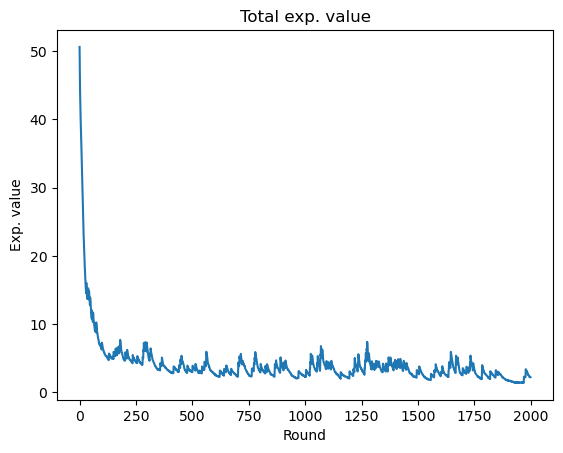
\includegraphics[width=0.45\textwidth]{chil-template-2023/images/avg_measured_exp_val.png}
    \caption{Expected value of $\ket{\psi}$ for the collapse - average game.}
    \label{fig:avg_measured_exp_val}
\end{figure}

\begin{figure}[h]
    \centering
    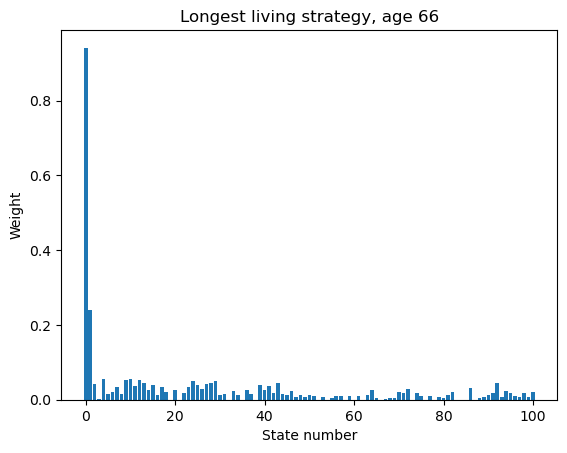
\includegraphics[width=0.45\textwidth]{chil-template-2023/Sections/avg_measured_oldest.png}
    \caption{Strategy with most rounds without an update (most rounds inside the elite).}
    \label{fig:avg_measured_oldest}
\end{figure}

For the results shown we again used $100$ players, $20$ elite players per round, $\pi = 0.5$, $\sigma = 0.05$ and $p = 0.5$. While a smaller $\pi$ leads to a decrease in the density of spikes seen in figure \ref{fig:avg_measured_exp_val}, a change to $\sigma = 0.1$ gives a non convergent game. We can therefore not find any value as a fix point. The noise is too strong for the convergence rate of the game. Interestingly this value seems to be somewhere in the region of a phase shift as for $\sigma = 0.09$ we can already see much better convergence with a lower bound of $\approx 9$.\\

\subsection{Weight of the Average: A Nonzero Equilibrium?}

With this approach we go back to using the average to determine $\ket{w}$ but we now determine the fitness from the weight each player assigned to the respective state $\ket{w}$.\\

This approach is particularly interesting as the winning players do not necessarily favor states with low averages but are only focused on the single state. This will eventually lead to a slower decay of the expected value. This is also enhanced by the mutation algorithm where the states not equal to $\ket{w}$ are uniformly distributed and only decrease in weight slowly, from the higher weight necessary on $\ket{w}$. Once the decay flattens we do not observe the expected value to reach a value around 0. Instead the expected value stays constant between 8 and 10, therefore giving $\ket{w}$ as $\ket{4}$ or $\ket{5}$. This only happens after some time by chance and shorter simulations often indicate a saturation between 10 and 12.\\

Additionally, we are able to observe large spikes of the expected value when inside a flat area. This may be caused by large mutations on higher states for multiple states in the elite, leading to a continuous boost of such features over the following rounds. An example for the course of the expected value is given in figure \ref{fig:single_avg_exp_val}.

\begin{figure}[h]
    \centering
    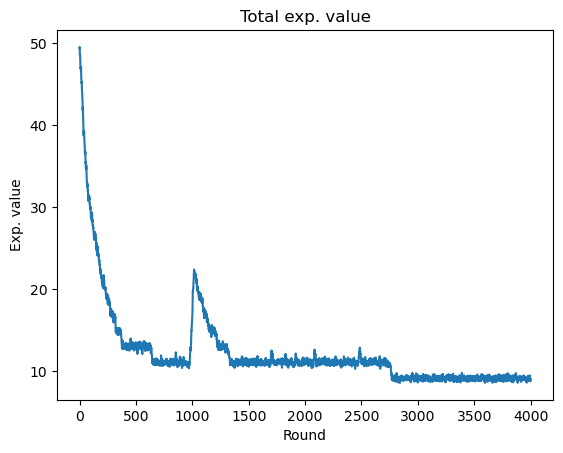
\includegraphics[width=0.45\textwidth]{chil-template-2023/images/single_avg_exp_val.png}
    \caption{Expected value of $\ket{\psi}$ for the weight of the average approach.}
    \label{fig:single_avg_exp_val}
\end{figure}

The reason for this behavior lies in the nonzero probability of higher states. Having a weight of $0.01$ on the state $\ket{100}$ increases the players expected value by $1$. As we have positive mutations on $25\%$ of the states as well as the remaining probabilities from the parents on higher states, an average of $0$ is, with the parameters as previously used in \ref{sub: The semi classical approach} and \ref{sub: Collapse with players average}, simply not possible.\\

For the exact point of convergence we were yet able to construct an exact formula but we do observe a linear scaling in $\sigma$. While the lower bound for $\sigma = 0.05$ was found to be 5, the lower bound for $\sigma = 0.01$ is determined to be 1. For such low sigma games, we also observe the establishment of dominant players which is again an effect of the mutation algorithm, although the mutations are already quite weak. Once a player finds a strategy with an almost pure 1 state, any mutation on other states leads to the a decrease in the weight of the 1 state and therefore looses against the dominant players. On the other hand, due to the rounding of $\ket{w}$, $\ket{0}$ is always a bad play if all or most players have some other non $\ket{0}$ state. We show the rounds won by each player after the saturation in figure \ref{fig:single_avg_times_won_at_1}, indicating the dominance of a few players.

\begin{figure}[ht]
    \centering
    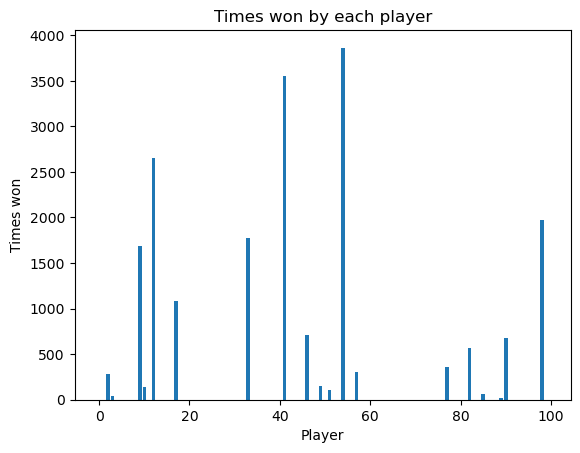
\includegraphics[width=0.45\textwidth]{chil-template-2023/images/single_avg_times_won_at_1.png}
    \caption{Times won by each player with $\sigma = 0.001$ and after boundary is reached.}
    \label{fig:single_avg_times_won_at_1}
\end{figure}

\subsection{The Projective Game}

In this approach we are using the projection of each player onto a state which is again determined by the collapse of $\ket{\psi}$ as already described in section \ref{sub: Collapse with players average}. In other words, the more likely a player is to receive the respective state upon measurement, the better its fitness. This game is quite complex for the player. For single rounds or rounds before a  clear convergence a player needs to have a good balance in their states. Distributing all probabilities evenly might not be enough to reach the elite. Putting all the weight on one card on the other hand kicks the player out of the elite for any other state. The second extreme is very much the same as betting all chips on one number at a roulette table but with a less significant reward if the state is actually found.\\

With the simulation we do find an area of uncertainty at the start of each game. With the two previous approaches we were more or less able to observe some kind of exponential decay in the expected value. With this approach on the other hand such a decay is only observed after many rounds were already played. Before that the game shows intervals of slower decay and even sections where the expected value may increase again. This behavior makes the decay already very much reliant on the seed for the random numbers which we were able to observe from decays starting after a wide range of rounds played. For our parameters this was generally still below 1000 rounds. Eventually the expected value still converges towards $\ket{0}$ were we again observe a similar behavior to the approach described in \ref{sub: Collapse with players average} with occasional spikes from non $\ket{0}$ measurements. By looking at the states $\ket{w}$ we can clearly see a phase transition from an unordered phase with many different winners to an ordered phase with only solitary non $\ket{0}$ measurements. The strategy surviving the most rounds even shows an almost pure $\ket{0}$ state with no weights above 0.1. Examples are shown in figures \ref{fig:single_measured_exp_val} - \ref{fig:single_measured_measured}.

\begin{figure}[h]
    \centering
    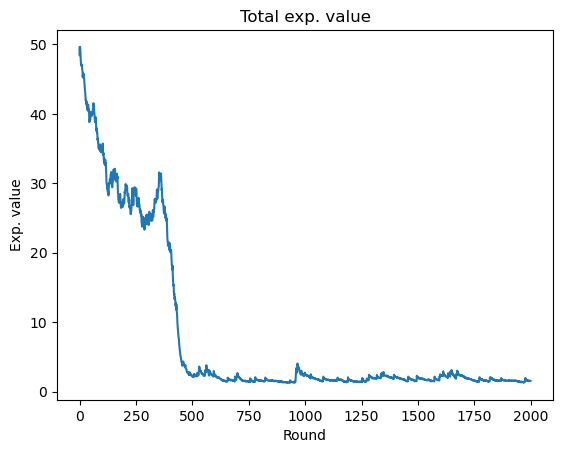
\includegraphics[width=0.45\textwidth]{chil-template-2023/images/single_measured_exp_val.png}
    \caption{expected value of $\ket{\psi}$ for the projection approach.}
    \label{fig:single_measured_exp_val}
\end{figure}

\begin{figure}[h]
    \centering
    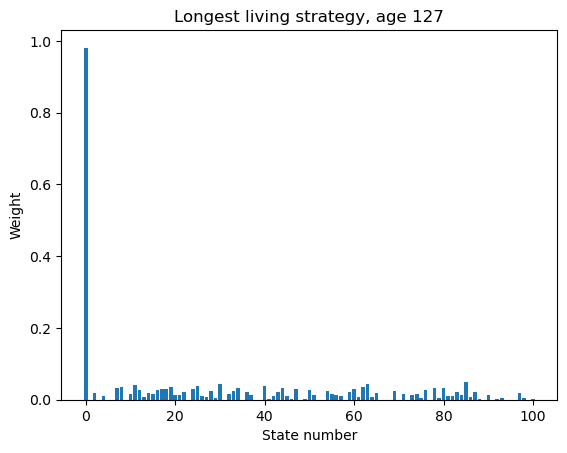
\includegraphics[width=0.45\textwidth]{chil-template-2023/images/single_measured_oldest.png}
    \caption{Longest living state for the projection approach.}
    \label{fig:single_measured_oldest}
\end{figure}

\begin{figure}[h]
    \centering
    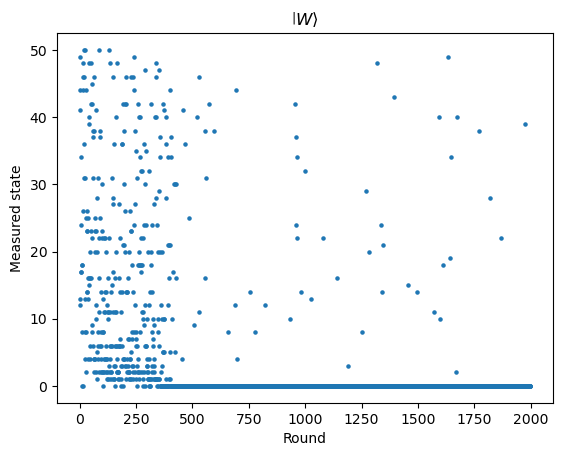
\includegraphics[width=0.45\textwidth]{chil-template-2023/images/single_measured_measured.png}
    \caption{Values of $\ket{w}$ over 2000 rounds for the projection approach.}
    \label{fig:single_measured_measured}
\end{figure}

For these results we used \texttt{np.random.seed(42)} and \texttt{np.random.seed(42)} with the first run of the simulation after setting the seed. The parameters are kept at the same values as before with $100$ players, $20$ elite players per round, $\pi = 0.5$, $\sigma = 0.05$ and $p = 0.5$. We again also try to bring up $\sigma$. Around $\sigma = 0.1$ we do not observe total chaos, as the longest living state is still dominated by $\ket{0}$ and the expected value is not distributed across all possible values. Still for $\sigma = 0.102$ we do see some form of oscillations over the course of $30.000$ rounds where we observe intervals with expected value around 15 as well as 40. At this point we do not have an explanation for this phenomena, especially why there still seems to be some order with two fix points and the system does not stabilize around $30$. What we also observe is a far more uniform distribution across all possible states in $\ket{w}$ when the expected value is around $40$ and far less measurements for states other than $\ket{0}$ when around $10$. This gives the indication that the game switches between relatively ordered and almost random states and large enough deviations from the mutation change the phase of the game. An example of this effect is shown in figure \ref{fig:single_measured_exp_val_0102}.

\begin{figure}[h]
    \centering
    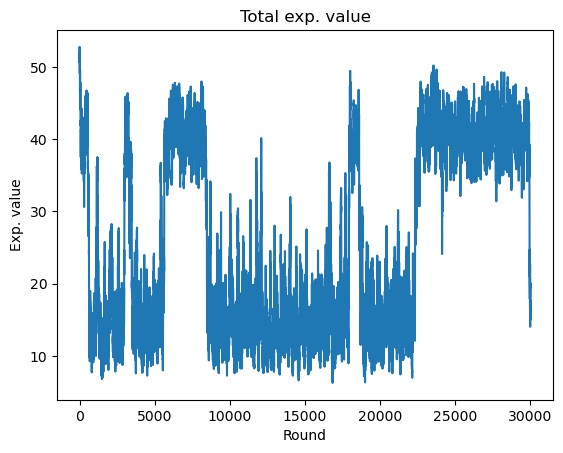
\includegraphics[width=0.45\textwidth]{chil-template-2023/images/single_measured_exp_val_0102.png}
    \caption{expected value of $\ket{\psi}$ for a simulation with on the projection game $\sigma = 0.102$.}
    \label{fig:single_measured_exp_val_0102}
\end{figure}

\subsection{Player Strategy Collapse}

Until now we have not looked at approaches where we collapsed each players strategy in order to determine the fitness score. The reason for this is simple: Using our previous approach of keeping the elite wave functions after a measurement not only seems to counter the idea of collapsing a wave function, it also leads to chaotic behavior where the expected value does not clearly converge to any point. This is regardless of determining $\ket{w}$ from the total expected value or also from a collapse of $\ket{\psi}$. Starting with almost uniform states the randomness which governs onto which state each player collapses is so large that good features (population of lower states) do not get the chance to become relevant. An example is shown if figure \ref{fig:measured_measured_exp_val}.\\

Changing the approach to setting the players strategy to its collapsed state before the next round as well as mutations does also not lead to any convergence in the expected value. Another possible change is to change the the order in the sense that we first collapse each players and then draw from the average. But even with this approach we do not see any convergence in the data again also trying out slight variations in the parameters.\\

This brings us to the conclusion that the confusion for the players is simply too large and for any described approach they are missing the incentive to develop a 'good' strategy in the sense of convergence.

\begin{figure}[h]
    \centering
    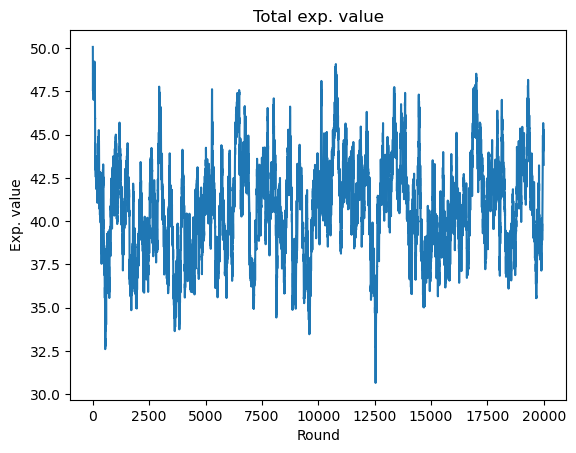
\includegraphics[width=0.46\textwidth]{chil-template-2023/images/measured_measured_exp_val.png}
    \caption{Example of a non convergent game based on wave function collapse of both $\ket{\psi}$ and all $\ket{S}$.}
    \label{fig:measured_measured_exp_val}
\end{figure}